\begin{figure}[H]
    \centering
    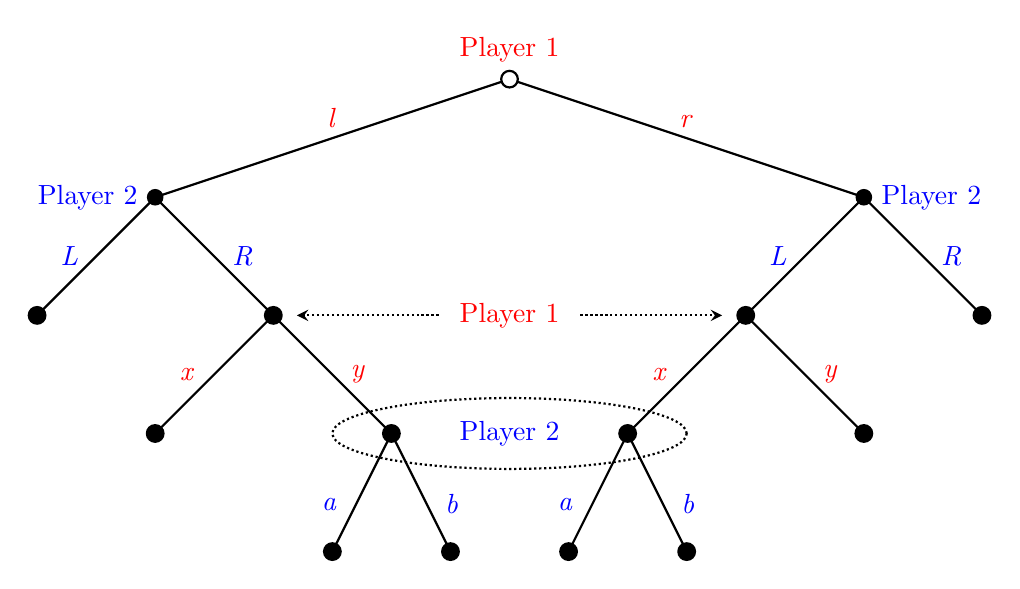
\begin{tikzpicture}[scale=1.5]
        % Player 1's first move
        \draw[thick] (0,0) -- (-3,-1) node[pos=.5,left,above] {\color{red}\textit{l}};
        \draw[thick] (0,0) -- (3,-1) node[pos=.5,right,above] {\color{red}\textit{r}};
        % Player 2's first move
        \draw[thick,fill] (-3,-1) -- (-4,-2) node[pos=.5,left=0.1cm] {\color{blue}\textit{L}} circle (2pt);
        \draw[thick,fill] (-3,-1) -- (-2,-2) node[pos=.5,right=0.1cm] {\color{blue}\textit{R}} circle (2pt);
        \draw[thick,fill] (3,-1) -- (2,-2) node[pos=.5,left=0.1cm] {\color{blue}\textit{L}} circle (2pt);
        \draw[thick,fill] (3,-1) -- (4,-2) node[pos=.5,right=0.1cm] {\color{blue}\textit{R}} circle (2pt);
        % Player 1's second move
        \draw[thick,fill] (-2,-2) -- (-3,-3) node[pos=.5,left=0.1cm] {\color{red}\textit{x}} circle (2pt);
        \draw[thick,fill] (-2,-2) -- (-1,-3) node[pos=.5,right=0.1cm] {\color{red}\textit{y}} circle (2pt);
        \draw[thick,fill] (2,-2) -- (1,-3) node[pos=.5,left=0.1cm] {\color{red}\textit{x}} circle (2pt);
        \draw[thick,fill] (2,-2) -- (3,-3) node[pos=.5,right=0.1cm] {\color{red}\textit{y}} circle (2pt);
        % Player 2's second move
        \draw[thick,fill] (-1,-3) -- (-1.5,-4) node[pos=.6,left=0.1cm] {\color{blue}\textit{a}} circle (2pt);
        \draw[thick,fill] (-1,-3) -- (-0.5,-4) node[pos=.6,right=0.1cm] {\color{blue}\textit{b}} circle (2pt);
        \draw[thick,fill] (1,-3) -- (0.5,-4) node[pos=.6,left=0.1cm] {\color{blue}\textit{a}} circle (2pt);
        \draw[thick,fill] (1,-3) -- (1.5,-4) node[pos=.6,right=0.1cm] {\color{blue}\textit{b}} circle (2pt);
        % Nodes and texts
        \draw[fill=white, thick] (0,0) circle[radius=2pt];
        \fill (-3,-1) circle (2pt) node[left=0.1cm] {\color{blue}Player 2};
        \fill (3,-1) circle (2pt) node[right=0.1cm] {\color{blue}Player 2};
        \draw[-stealth, densely dotted, thick] (-0.6,-2) -- (-1.8,-2);
        \draw[-stealth, densely dotted, thick] (0.6,-2) -- (1.8,-2);
        \node at (0,-2) {\color{red}Player 1};
        \node[above=0.1cm] at (0,0) {\color{red}Player 1};
        \draw[densely dotted, thick] (0,-3) ellipse (1.5cm and 0.3cm);
        \node at (0,-3) {\color{blue}Player 2};
    \end{tikzpicture}
\end{figure}